% Report
\documentclass[10pt,journal]{IEEEtran}

% Packages
\usepackage{amsfonts}
\usepackage{amsmath}
\usepackage{algorithm}
\usepackage{algorithmic}
\usepackage{amssymb}
\usepackage{graphicx}
	\graphicspath{{F:/校文件/数学/概率论/Project/Figures/}}
\usepackage{cite}
\usepackage{subfigure}
\usepackage{float}
\usepackage{color}
\usepackage[colorlinks, linkcolor = red]{hyperref}

\begin{document}

% Title
\title{Algorithmic Mechanism Modeling of WeChat Red Envelope Game}
\author{\IEEEauthorblockN{Guanzhou Hu}\\
\IEEEauthorblockA{School of Information Science and Technology\\
  ShanghaiTech University}} 
\maketitle

% Abstract
\begin{abstract}
This report focuses on the analysis and simulation of stochastic algorithmic mechcanism behind WeChat Red Envelopes. In the first stage, data of two hundred trials are produced and collected, followed by a comprehensive analysis. Next, two different hypotheses (including static mechanisms and dynamic algorithms) are proposed based on analytic results, which then go through a mathematical verification. Sequentially, both verified algorithms are realized by a \textit{Python} program. Simulation results will get analyzed and compared with real data, in order for a hypotheses testing. A good approximation of WeChat Red Envelope algorithm will finally get put forward.
\end{abstract}

% Introduction
\section{Introduction}
WeChat Red Envelope is a popular social game based on WeChat Platform. It gains popularity mainly from its randomness. The sender plugs in a certain amount of money $m$ into a virtual red envelope, sets the restriction of envelope size $n$ - the number of people that can open this envelope, and sends it into a chat group. Members in the group can open this envelope and grab a random amount of money, as long as the limitation of number of people is not exceeded. \\

The main results and contributions of this report are summarized as follows:
\begin{itemize}
  \item \textbf{A proper modeling of red envelope algorithm.}
  \item \textbf{Mathematical analysis of red envelope mechanism.}
  \item \textbf{Simulation results of virtual red envelope games.}
\end{itemize}

% Data Analysis
\section{Data Analysis}
Dataset is generated within two chat groups of $36$ members in total. Red envelope size is fixed as [Amount $m = 10$ Yuan / Number of people $n = 10$] during the analysis stage, in the purpose of regulation and normalization of data. Based on overall $202$ pieces of valid data, the following analyses are conducted:
%% Mean and Variance
\subsection{Mean and Variance at Positions}
For each red envelope with size [$10$ Yuan / $10$], denote the order of snatching as position $0, 1, \dots , 9$. Let $A_i$ be the amount of money that is grabbed by position $i, i \in \{0, 1, \dots , 9\}$, therefore $\sum_{i=0}^9 A_i = 10$ for each envelope. The \textit{mean} and \textit{variance} of $A_i$ shows great uniformity among different positions, as shown in Figure \ref{fig:data1}.
\begin{figure}[H]
	\centering
	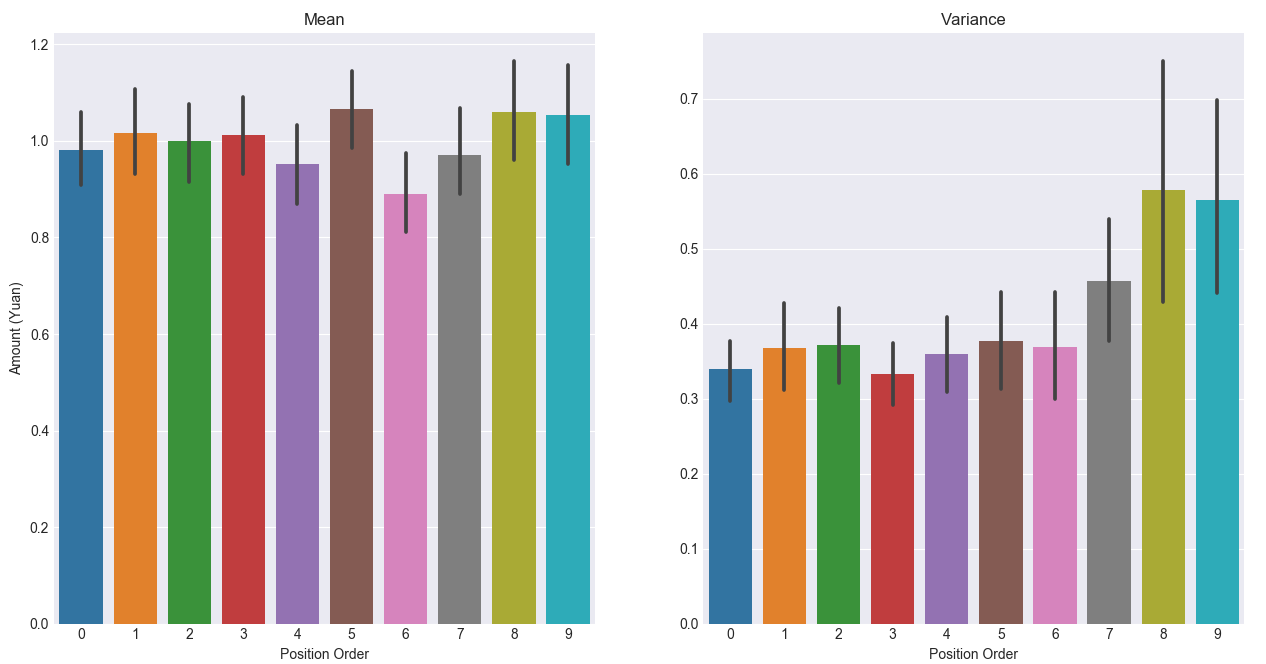
\includegraphics[width=0.95\columnwidth]{data1.png}
	\caption{Mean and Variance at Positions} \label{fig:data1}
\end{figure}
Notice that the variance at latter positions are generally larger.
%% Distribution
\subsection{Distribution at Positions}
At each position $i$, distribution of the amount grabbed $A_i$ is shown in Figure \ref{fig:data2}.
\begin{figure}[H]
	\centering
	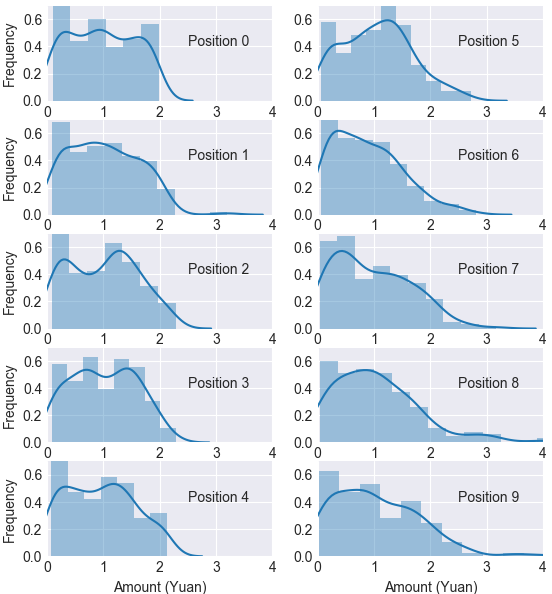
\includegraphics[width=0.95\columnwidth]{data2.png}
	\caption{Distribution at Positions} \label{fig:data2}
\end{figure}
The amount of money $A_i$ snatched by the person at position $i$ approximately follows a Uniform distribution for smaller order positions, and a truncated Normal distribution $\mathcal{N}_T(\mu_i, \sigma_i)$ for latter positions.
%% Max and Min
\subsection{Max and Min Amount in Envelopes}
The Max and Min amount of money grabbed in each red envelope are plotted in Figure \ref{fig:data3}.
\begin{figure}[H]
	\centering
	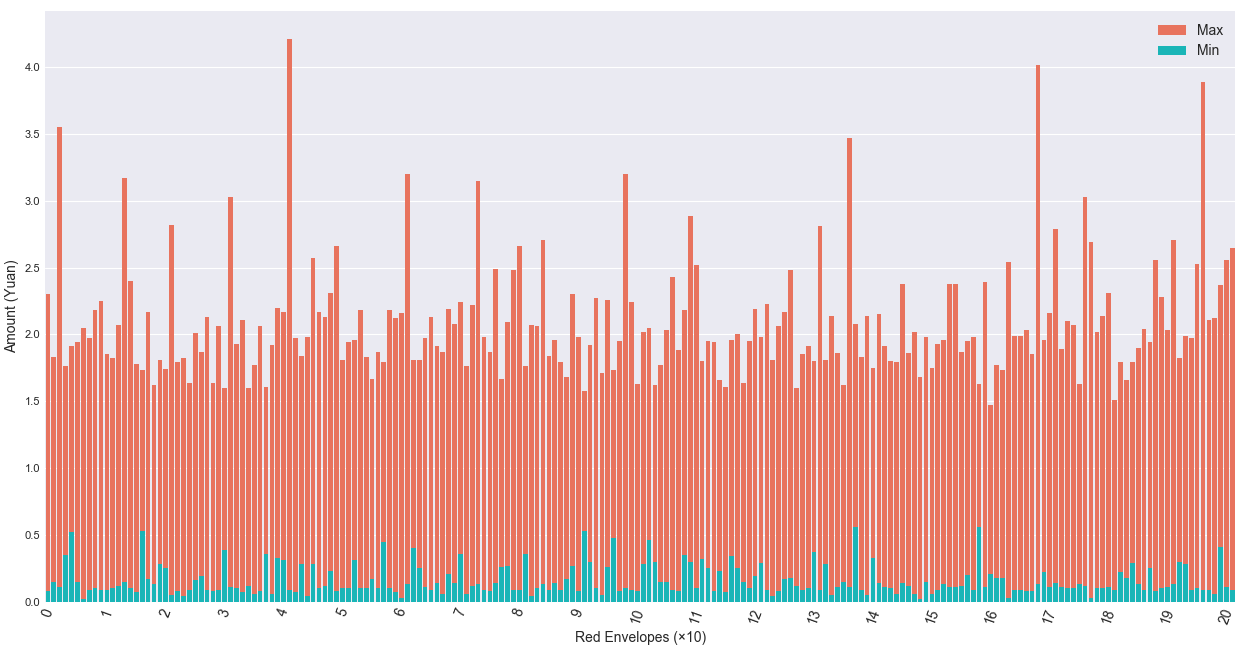
\includegraphics[width=0.95\columnwidth]{data3.png}
	\caption{Max and Min of Envelopes} \label{fig:data3}
\end{figure}
The Maximum amount of money in each red envelope is generally larger than $1.5$ Yuan, and smaller than $2.0$ Yuan, except for some outstanding peaks which reach the largest value of $4.21$ Yuan. The Minimum amount is generally smaller than $0.5$ Yuan, and touches the smallest possible value of $0.01$ Yuan in some envelopes.

% Model Hypotheses
\section{Model Hypotheses}
The analytic result of collected red envelope data reveals the following five significant insights:
\begin{enumerate}
	\item \textbf{Each position has a generally stable mean around $m/n = 1$.}
	\item \textbf{Variance is slightly increasing, and shows a large jump at the penultimate position.}
	\item \textbf{Smaller order positions, especially the first position, reveal an Uniform distribution, meanwhile the latter positions show a truncated Normal distribution.}
	\item \textbf{The Min amount of money basically ranges from $0.01$ Yuan to $0.5$ Yuan, and has the possibility of touching the very bottom.}
	\item \textbf{The Max amount of money basically ranges from $1.5$ Yuan to $2.0$ Yuan, and has the possibility of reaching a respectively large value of over $4.0$ Yuan.}
\end{enumerate}
Based on these five observations, the following two hypotheses of algorithm models are proposed and will be examined mathematically. 
%% STATIC
\subsection{Static-Uniform Model}
Suppose the allocation of money inside every red envelope is completely computed at the exact sending time. The envelope seen by chat group members is simply static, offline package of numbers. Every time the envelope is snatched, it returns a uniformly randomly chosen number inside the package. See Figure \ref{fig:model1} for an illustration.
\begin{figure}[H]
	\centering
	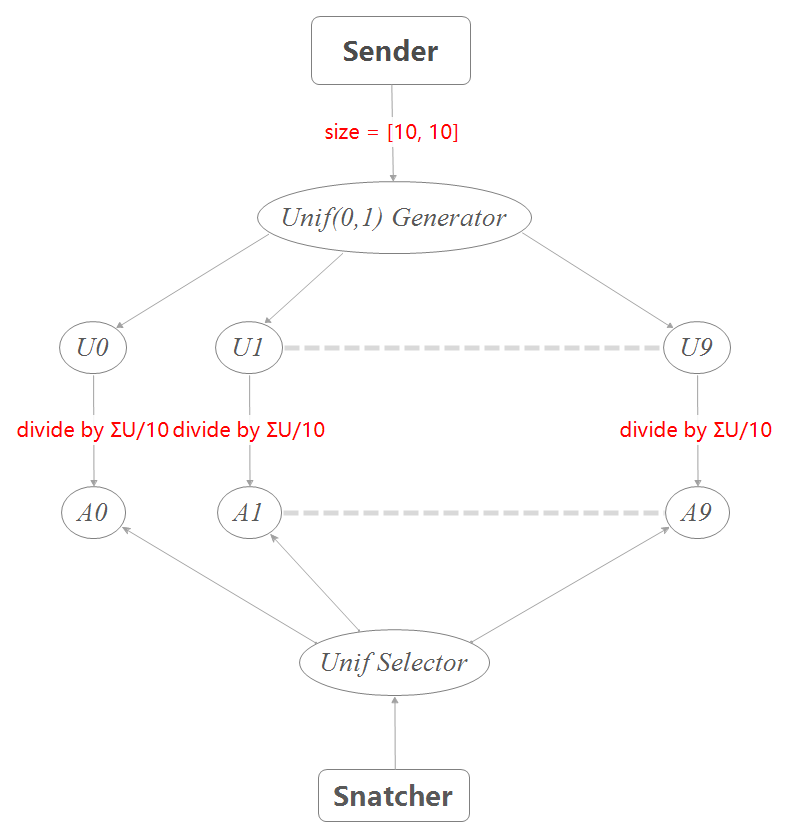
\includegraphics[width=0.95\columnwidth]{model1.png}
	\caption{Static-Uniform Model} \label{fig:model1}
\end{figure}
Consider $m = n = 10$ cases, denote random variables $A_i$ as stated above, $i \in \{0, 1, \dots ,9\}$. According to the symmetry and linearity of expectations, we have
\[
	E(A_i) = \frac{E(\sum_{j=0}^{9} A_j)}{10} = 1
\]
for all $i \in \{0, 1, \dots ,9\}$, which corresponds to insight 1). Since $U_0, U_1, \dots , U_9 \sim$ Unif($0, 1$), the $j$th order statistics $U_{(j)} \sim$~Beta($j, 10-j+1$). Therefore, the Max and Min value $U_{max}$ and $U_{min}$ satisfies
\[
	P(U_{min} \le 0.25) = P(U_{(1)} \le 0.25) \approx 0.947
\]
\[
	P(U_{max} \ge 0.75) = P(U_{(10)} \ge 0.75) \approx 0.947
\]
which agrees with insight 4) and 5), since the expected scaling ratio between $A_i$ and $U_i$ is now $E(A_i)/E(U_i) = 2$. \\

This model does not satisfy insight 2) and 3) well, however is already a good approximation and is worthy being simulated.
%% DYNAMIC
\subsection{Dynamic-Updating Model}
Suppose the amount of money snatched from the red envelope is generated dynamically at the time when a member opens it. Under this scenario, the amount of money $A_0 A_1, \dots ,A_9$ grabbed by different positions are dependant with each other. Therefore, every generating of $A_i$ is influenced by its position $i$ and the rest money $m_i'$. A significant restriction that might get neglected is that every person should at least grab $0.01$ Yuan, therefore when the algorithm reaches the stage $A_8$, it needs some adjustments to ensure $A_9 \ge 0.01$. See Figure \ref{fig:model2} for an illustration.
\begin{figure}[H]
	\centering
	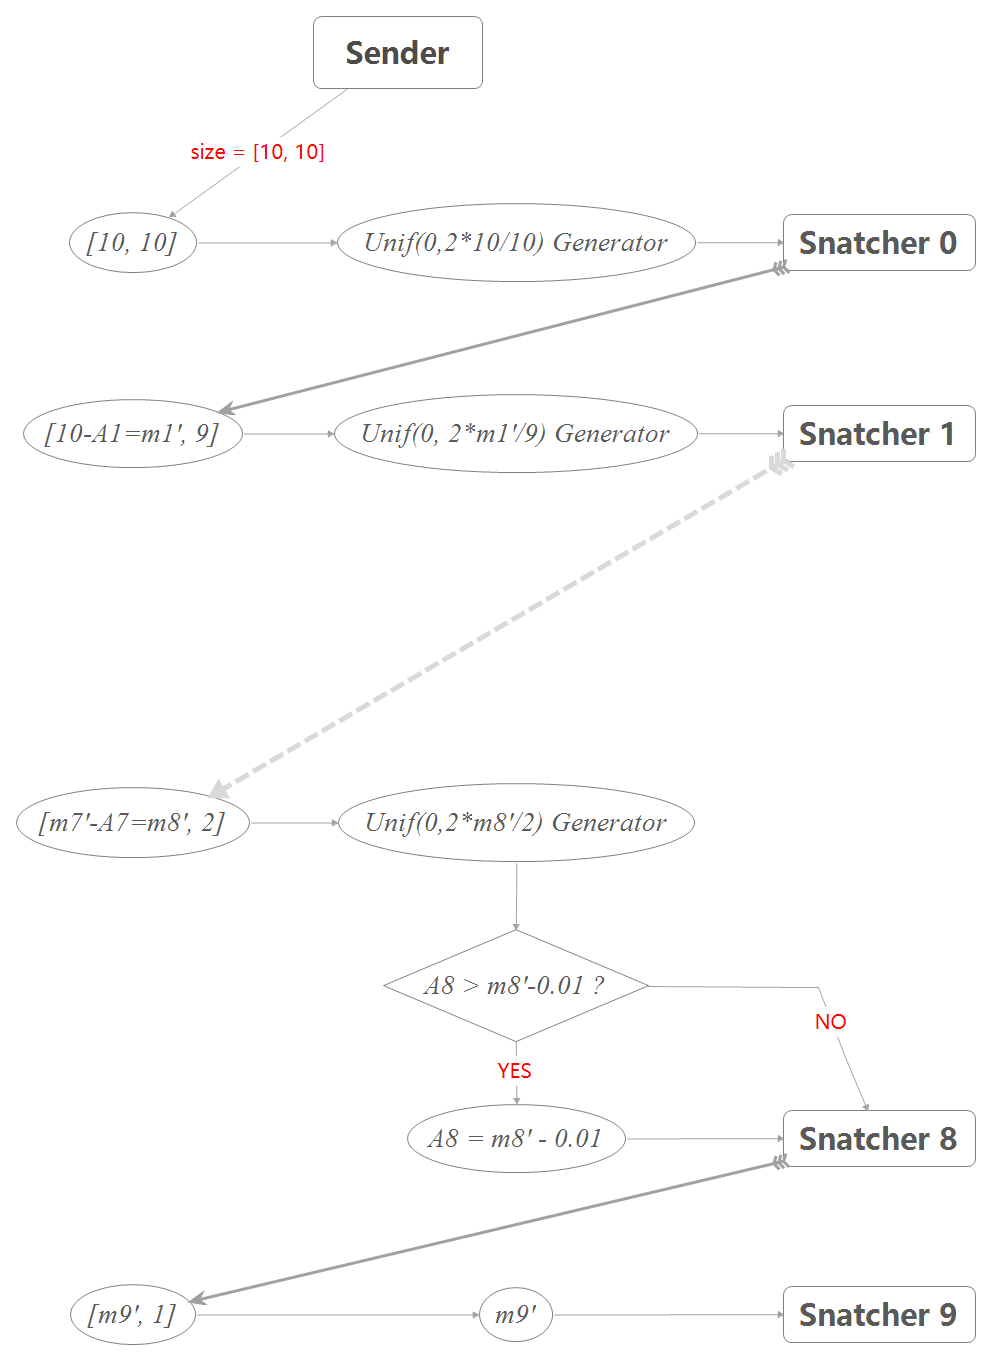
\includegraphics[width=0.95\columnwidth]{model2.png}
	\caption{Dynamic-Updating Model} \label{fig:model2}
\end{figure}
This algorithm always generates a uniformly random amount of money ranging from $0.01$ Yuan to twice the mean of the rest red envelope. For the first position, $A_0 \sim$ Unif($0, 2\frac{m}{n}$), we have
\[
	E(A_0) = \frac{0 + 2 \times \frac{m}{n}}{2} = \frac{0 + 2 \times \frac{10}{10}}{2} = 1
\]
Conditioning on the first position, $A_1|A_0 = a \sim$ Unif($0, 2\frac{m-a}{n-1}$). So according to Adam's Law, for the position 1, we have
\begin{equation*} \begin{aligned}
	E(A_1) &= E(E(A_1|A_0)) \\
		&= E(\frac{10 - A_0}{9}) \\
		&= \frac{10 - E(A_0)}{9} \\
		&= 1
\end{aligned} \end{equation*}
and similar for the rest positions. Therefore it corresponds to insight 1). The variance of $A_0$ is
\[
	Var(A_0) = \frac{(2-0)^2}{12} = \frac{1}{3}
\]
and according to Eve's Law, the variance of $A_1$ at position 1 will be
\begin{equation*} \begin{aligned}
	Var(A_1) &= E(Var(A_1|A_0)) + Var(E(A_1|A_0)) \\
		&= E(\frac{(2 \frac{10 - A_0}{9} - 0)^2}{12}) + Var(\frac{10 - A_0}{9}) \\
		&= \frac{100}{243} - \frac{20}{243} E(A_0) + \frac{1}{243} E(A_0^2) + \frac{1}{81} Var(A_0) \\
		&= \frac{247}{9^3} \approx 0.339 > \frac{1}{3} = Var(A_0)
\end{aligned} \end{equation*}
which agrees with the increasing variance in insight 2). Also, as the result of extra adjusting at position 8, $A_8$ and $A_9$ suffers more uncertainty than previous positions, which perfectly answers the jump of variance at position 8. The truncated Normal distribution at latter positions is also a natural consequence under this model. Detailed proof will be omitted.

% Simulation
\section{Simulations and Testing}
Simulation programs of both Static-Uniform model and Dynamic-Updating model are accomplished using \textit{Python} language. In order to conduct hypotheses testing, both programs are run with the same size of red envelope $[10, 10]$ and the same number of samples $202$. After acquiring the simulation results, the following three targets are evaluated and compared to the original data:
\begin{itemize}
	\item \textbf{Uniformity of Mean}
	\item \textbf{Regression Curve of Variance}
	\item \textbf{Probability Distribution at Positions}
\end{itemize}
%% Uniformity of Mean
\subsection{Uniformity of Mean}
The mean values of amount of money $A_0, A_1, \dots , A_9$ from original raw data and two simulation models are shown in Figure \ref{fig:result1}.
\begin{figure}[H]
	\centering
	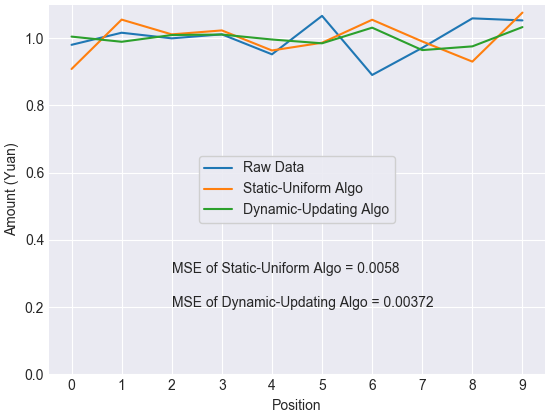
\includegraphics[width=0.95\columnwidth]{result1.png}
	\caption{Comparing Uniformity of Mean} \label{fig:result1}
\end{figure}
Denote $\tilde{A_i}$ to be the mean values of raw data, and $\hat{A_i}$ to be the mean values of simulated data, for $i \in \{0, 1, \dots ,9\}$. Mean square error (MSE) of simulation results compared to raw data is defined as
\[
	MSE = \frac{1}{10} \sum_{j=0}^9 (\hat{A_j} - \tilde{A_j})^2
\]
which represents the deviation of mean values from raw data. As computed, $MSE$ of Dynamic-Updating model $\approx 0.00372$, while $MSE$ of Static-Uniform model $\approx 0.00580$. This reveals that the Dynamic-Updating model generally performs better than Static-Uniform model on approximating mean values.
%% Variance Regression
\subsection{Variance Regression}
The variance of $A_0, A_1, \dots , A_9$ are sampled and estimated using an order-$2$ regression. The regression plot in shown in Figure \ref{fig:result2}.
\begin{figure}[H]
	\centering
	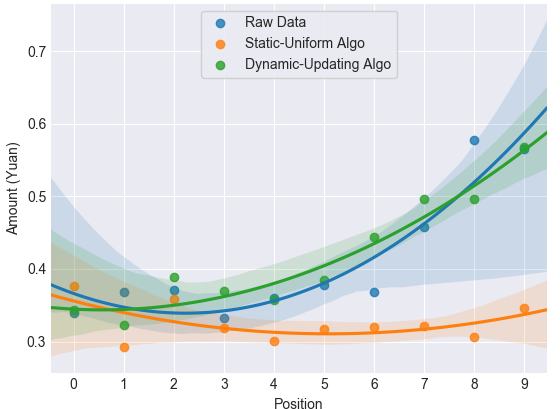
\includegraphics[width=0.95\columnwidth]{result2.png}
	\caption{Comparing Variance Regression} \label{fig:result2}
\end{figure}
It can be observed that the output of Dynamic-Updating model follows a perfect regression curve, meanwhile the Static-Uniform model does not reproduce the increasing and jumping variance. Therefore, Dynamic-Updating model performs much better than Static-Uniform model on approximating the fluctuation of amount of money.
%% Distribution at Positions
\subsection{Distribution at Positions}
The distribution of $A_0, A_1, \dots , A_9$ are from original raw data and two simulation models are shown in Figure \ref{fig:result3}.
\begin{figure}[H]
	\centering
	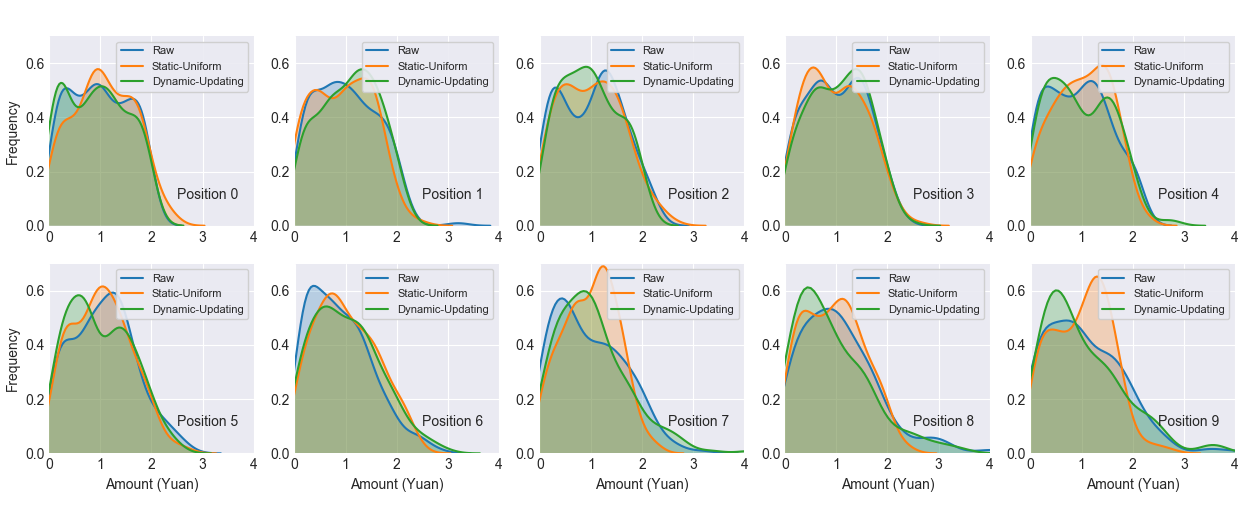
\includegraphics[width=0.95\columnwidth]{result3.png}
	\caption{Comparing Distribution at Positions} \label{fig:result3}
\end{figure}
Both Static-Uniform and Dynamic-Updating models perform well in approximating distributions at different positions. However, Static-Uniform algorithm does not reveal the Uniform distribution at earlier positions and the truncated Normal distribution at latter positions as clearly as Dynamic-Updating algorithm. Therefore, Dynamic-Updating model still performs better than Static-Uniform model on approximating the distribution at each position.

% Conclusions
\section{Conclusions}
In summary, the Dynamic-Updating model is a perfect approximation of the Wechat Red Envelope algorithm mechanism. It is an online algorithm that generates a uniformly random amount of money ranging from $0.01$ Yuan to twice the mean of rest envelope $2\frac{m_i'}{n-i}$. It satisfies the uniformity of mean and the increasing variance along the positions, and especially answers the jump of variance at the penultimate position.\\

Further works, including tests on different sizes of data other than $[10, 10]$, and optimization of this algorithm on lightening the server load, still need to be done.

% Acknowledgment
\section*{Acknowledgment}
During this project, I collaborated and discussed with my classmates Xinyu Zhang, Ruoyu Wang, Zikun Xiao and Haoyi Zhu. I also adopted part of contents from Zhihu \cite{Zhihu1} \cite{Zhihu2} to Section III about the idea of dynamic algorithm mechanism. Original red envelope data is collected in two chat groups on WeChat with in total 36 student members. I appreciate Ruoyu Wang and Yuyan Zhou for helping to collect the raw data.

% References
\bibliographystyle{IEEEtran}
\bibliography{Reference}

\end{document}
